\section{Analisi dei Risultati}
\label{section:analisirisultati}

Prima di iniziare ad elencare i test effettuati e mostrare i risultati ottenuti, è
necessario sottolineare una questione relativamente importante:
in seguito all'osservazione del comportamento dell'applicativo con grafi molto grandi (> 500 nodi) è stato ritenuto opportuno
abbassare il numero dei nodi affinchè l'esecuzione non impiegasse troppo tempo e risorse.
In conclusione tutte le analisi sono state effettuate con reti composte da 500 nodi.
Un secondo punto da chiarire è che avendo due applicativi, 
il primo in Java che punta a creare grafi (Capitolo~\ref{section:graph_topologies_dm}) 
ed il secondo in NetLogo che mira ad utilizzarli nelle simulazioni,
è stato ritenuto opportuno non cambiare mai il grafo durante i test.

\vspace*{-5pt}
\subsection{Primo test}
\label{section:first_test}

In questa prima analisi verranno confrontati i due tipi di grafo descritti nel capitolo \ref{section:graph_topologies}.

Per questo test abbiamo bisogno di alcuni elementi imprescindibili, tali:
\begin{itemize}
\vspace*{-3pt}
\item un gruppo di utenti che forma il 100\% dei nodi;
\item un grafo di 500 nodi creato grazie all'algoritmo Preferential Attachment (Capitolo \ref{section:graph_topologies_pa});
\item un grafo di 500 nodi creato grazie all'algoritmo di Dorogovtsev e Mendes (Capitolo \ref{section:graph_topologies_dm});
\item un ciclo che vari la ``forza'' della notizia portandola da 0 a 1 con passi di 0.05.
\end{itemize}


\begin{figure}[!ht]
  \begin{subfigure}[l]{0.5\textwidth}
    \begin{center}
      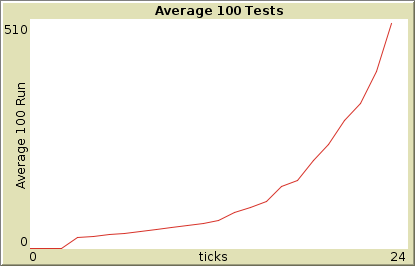
\includegraphics[width=1\textwidth, height=35mm]{img/interface-test-1-preferential-attachment-chart.png}
    \end{center}
    \caption{Con Preferential Attachment}
    \label{img:result_test_1_pa}
  \end{subfigure}
  \begin{subfigure}[r]{0.5\textwidth}
    \begin{center}
      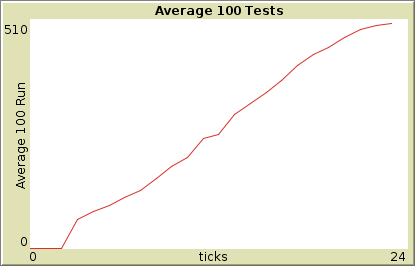
\includegraphics[width=1\textwidth, height=35mm]{img/interface-test-1-dorogovtsev-mendes-chart.png}
    \end{center}
    \caption{Con Dorogovtsev e Mendes}
    \label{img:result_test_1_dm}
  \end{subfigure}
 \caption{Risultati del primo test}
 \label{img:results_test_1}
 \vspace*{-10pt}
\end{figure}


Grazie al grafo descritto da Barabási e Albert si ottiene il risultato mostrato nel grafico di figura \ref{img:result_test_1_pa}, 
come è possibile notare, in questo caso, si avrà una crescita molto lenta e solo dopo che la probabilità di condivisione avrà 
superato il valore di 0.5 si otterà un aumento tangibile.
La topologia descritta da Dorogovtsev e Mendes, invece, mostra un comportamento differente come da grafico in figura \ref{img:result_test_1_dm}, 
si evidenzia una crescita quasi lineare e alla fine, quando la forza è attorno l'85\% crea una ``pancia'' verso l'alto, a dimostrare l'altissima 
condivisione.

Il primo grafo risulta essere svantaggiato per via della sua struttura, come affermato  
in fase di progettazione (Capitolo \ref{section:progettazione}) questo grafo non presenta cricche al suo interno.
Le proprietà appena descritte rappresentano una "penalità" sulla probabilità di condivisione per le simulazioni basate sul numero di visualizzazioni. 
Il modello descritto da Dorogovtsev e Mendes invece presenta cricche ed il grafo di questo esempio ne è la prova; 
esso ha infatti quasi il doppio dei link del Preferential Attachment.

Considerato quanto appena esposto, il confronto tra i due modelli di grafo ci permette di desumere come la seconda topologia 
affronti in maniera più migliore questo studio.
Si è perciò optato di sostenere i prossimi test con la seconda topologia realizzata da Dorogovtsev e Mendes.

Inoltre, nonostante si tratti solo del punto di vista dell'autore, nel seguente modello di grafo si può notare una 
maggior somiglianza con la topologia più comune di un Social Network.

\subsection{Secondo test}
\label{section:second_test}

In seguito al confronto studiato nel primo test, ed aver deciso quale fosse il modello di grafo migliore per questo tipo di analisi, 
è possibile concentrarsi sulla seconda fase definita degli obiettivi.
Questo secondo studio permetterà di analizzare la modalità di condivisione di una notizia, con un argomento, in differenti 
Social Network\footnote{\scriptsize Per Social Network viene inteso lo stesso grafo di 500 nodi utilizzato in precedenza 
ma con le età degli utenti prese dallo studio statistico di figura~\ref{img:age_distribution_social}.}.
La notizia ha 5 valori di forza di condivisione che si riferiscono ai 5 differenti gruppi di età. 
La prima prova ha implicato l'inizializzazione dei valori di forza, di tutti i gruppi tranne che per quello con più utenti, a
0.75\footnote{\scriptsize 0.75 è un valore piuttosto alto che permette una buona condivisione.}.
Quest'ultimo infatti verrà fatto variare da 0 a 1 con passi di 0.05.
Ci permetterà di capire come cambiano i ``Viewers'' in queste condizioni.

\begin{figure}[!ht]
  \begin{subfigure}[l]{0.32\textwidth}
    \begin{center}
      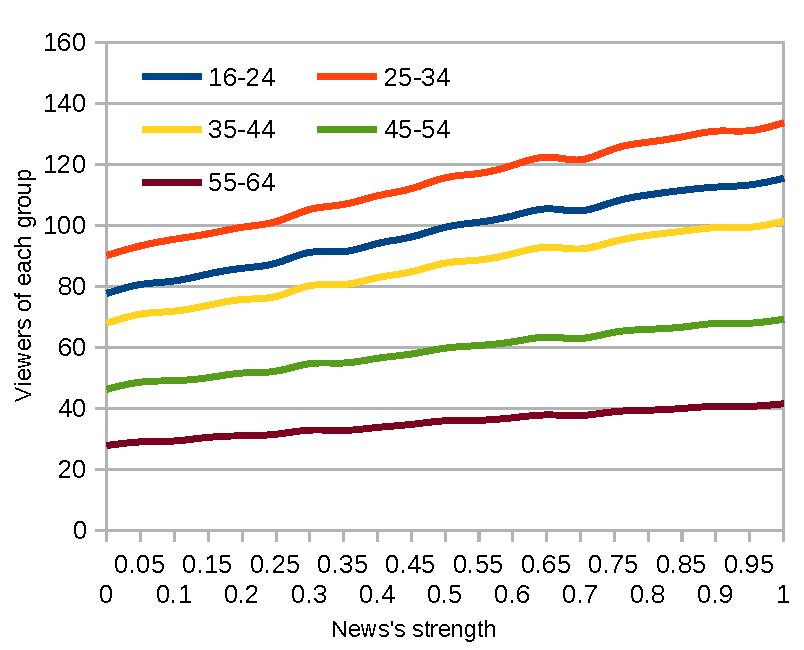
\includegraphics[width=1\textwidth]{charts/second-test-fb_1.pdf}
    \end{center}
    \vspace*{-10pt}
    \caption{Facebook}
    \label{img:result_test_2_fb_1}
  \end{subfigure}  
  \begin{subfigure}[c]{0.32\textwidth}
    \begin{center}
      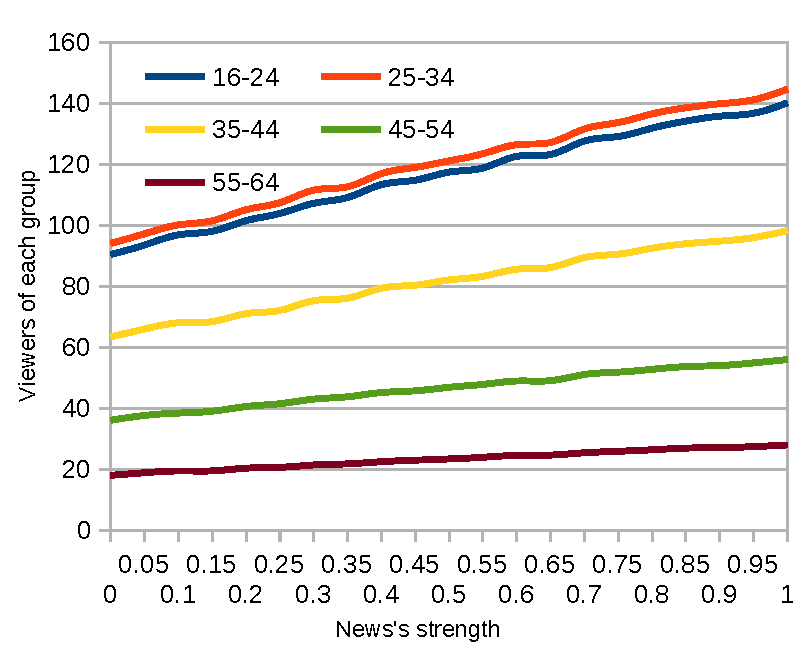
\includegraphics[width=1\textwidth]{charts/second-test-tw_1.pdf}
    \end{center}
    \vspace*{-10pt}
    \caption{Twitter}
    \label{img:result_test_2_tw_1}
  \end{subfigure}  
  \begin{subfigure}[r]{0.32\textwidth}
    \begin{center}
      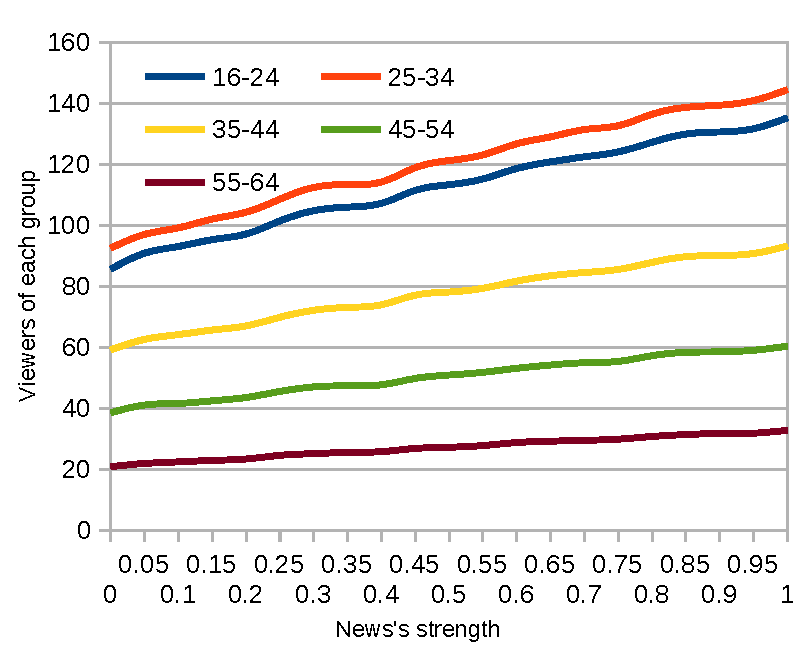
\includegraphics[width=1\textwidth]{charts/second-test-gp_1.pdf}
    \end{center}
    \vspace*{-10pt}
    \caption{Google+}
    \label{img:result_test_2_gp_1}
  \end{subfigure}  
 \caption{Risultati del secondo test}
 \label{img:results_test_2_1}
\vspace*{-15pt}
\end{figure}

Nei grafici di figura~\ref{img:results_test_2_1} si nota un'alta linearità con le percentuali di età definite nel social Network, 
mentre la crescita risulta dovuta dall'aumento progressivo della forza di condivisione della notizia.
Le curve nei grafici non partono dall'origine poichè il valore 0.75 fornisce una buona condivisione, sebbene non ottima; 
sommando questi ultimi infatti, l'ottimo, ovvero le 500 condivisioni, non viene mai raggiunto.

Per testare la linearità del grafo è stato prodotto un secondo test dove, a differenza di quello appena compiuto,
verranno variati tutti e 5 i valori di forza da 0 a 1.


\vspace*{-15pt}
\begin{figure}[!ht]
  \begin{subfigure}[l]{0.32\textwidth}
    \begin{center}
      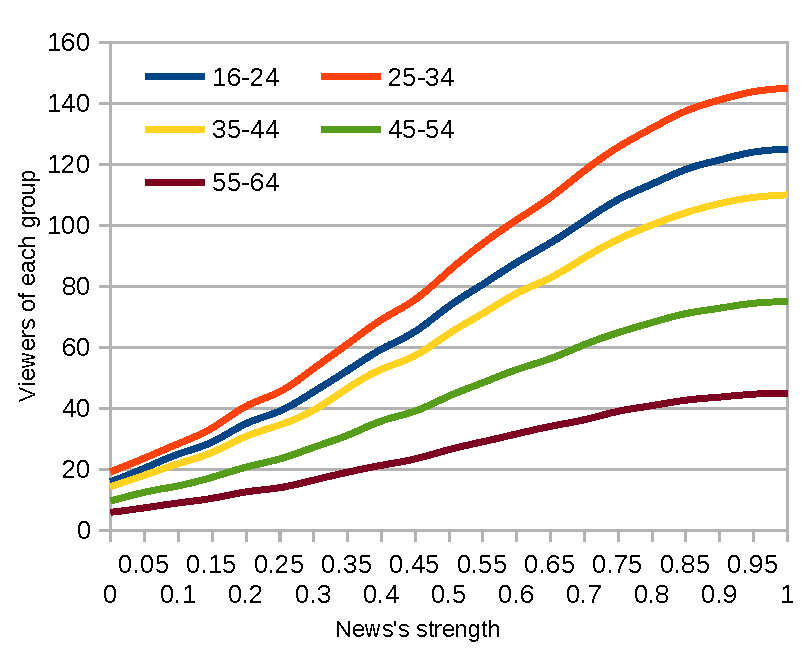
\includegraphics[width=1\textwidth]{charts/second-test-fb_2.pdf}
    \end{center}
    \vspace*{-10pt}
    \caption{Facebook}
    \label{img:result_test_2_fb_2}
  \end{subfigure}  
  \begin{subfigure}[c]{0.32\textwidth}
    \begin{center}
      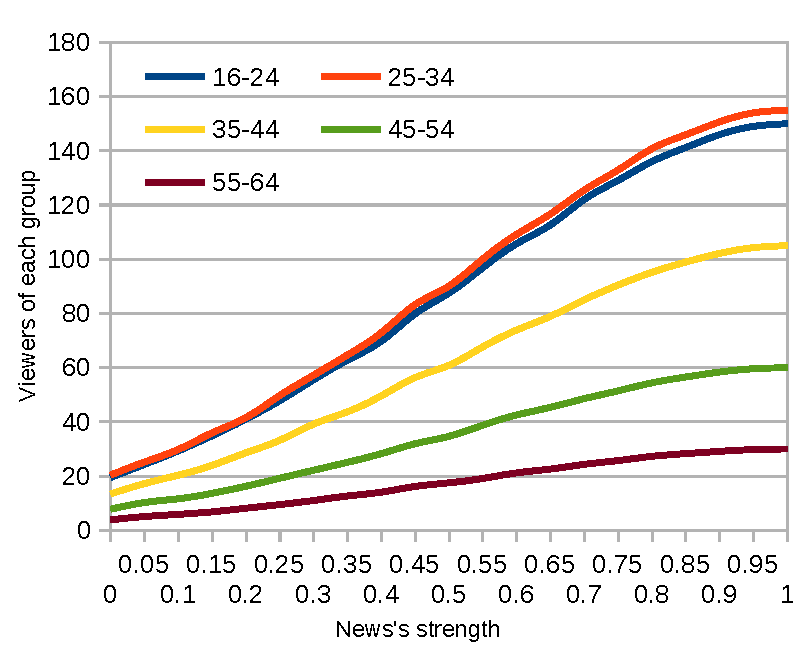
\includegraphics[width=1\textwidth]{charts/second-test-tw_2.pdf}
    \end{center}
    \vspace*{-10pt}
    \caption{Twitter}
    \label{img:result_test_2_tw_2}
  \end{subfigure}  
  \begin{subfigure}[r]{0.32\textwidth}
    \begin{center}
      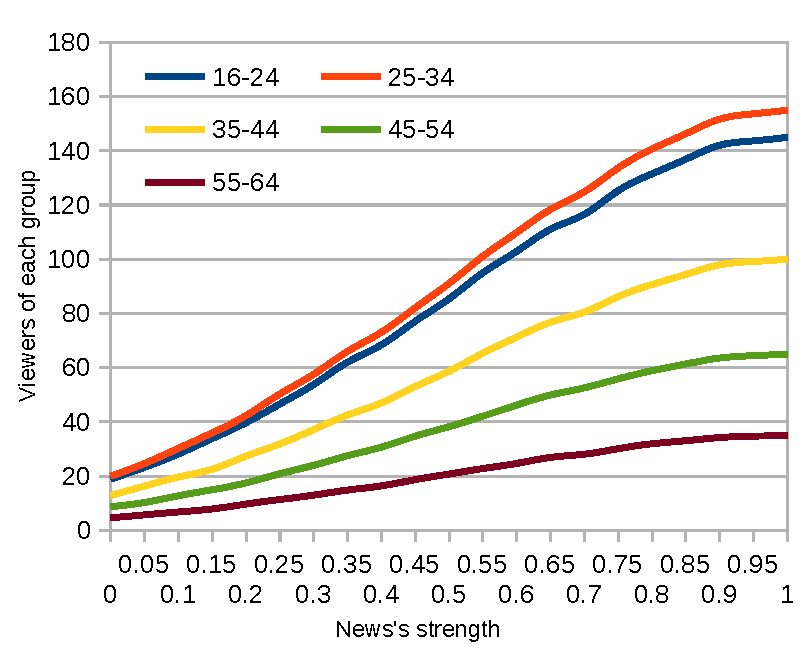
\includegraphics[width=1\textwidth]{charts/second-test-gp_2.pdf}
    \end{center}
    \vspace*{-10pt}
    \caption{Google+}
    \label{img:result_test_2_gp_2}
  \end{subfigure}  
 \caption{Risultati del secondo test}
 \label{img:results_test_2_2}
\end{figure}
\vspace*{-15pt}

I grafici di figura~\ref{img:results_test_2_2} confermano la crescita lineare dovuta dall'aumento della forza per tutti i gruppi.
Anche in questo caso è possibile osservare la stessa "pancia" verso l'alto, vista nel grafico di figura~\ref{img:result_test_1_dm}. 
Si vuole inoltre far notare come, al passo 0, le visualizzazioni siano differenti da 1 ovvero quella del paziente zero.
Il motivo è semplice, infatti, tutti quei nodi direttamente connessi al primo condivisore diventano ``Viewers''.

\subsection{Terzo test}
\label{section:third_test}

In quest'ultima analisi, invece, verrà mostrata un'interazione tra 2 diversi gruppi di utenti (Nodi):
il primo gruppo sarà formato da persone con una maggior probabilità di condividere la notizia 
mentre nel secondo, al contrario, da persone con una minor probabilità.
Questo studio punta ad analizzare quante visualizzazioni vengono fatte per una singola informazione condivisa.
In seguito verrà poi condotto uno studio in cui il totale degli utenti si dividerà in due gruppi costituiti da, ad esempio, 
pochi utenti con alte probabilità di condividere l'informazione e, viceversa, 
molti utenti con basse probabilità di condivisione.

La possibilità di condivisione sarà data nuovamente dal confronto tra la ``forza della notizia'' e la ``forza di astensione''. 
In questo caso, però, l'astensione verrà calcolata tramite una funzione di distribuzione di probabilità non lineare,
quella scelta è la funzione Weibull già descritta al capitolo~\ref{section:great_sharers_vs_little_sharers}.

Per ottenere una curva di distribuzione più o meno inclinata, in seguito ai tentativi attuati, 
è stato ritenuto opportuno mantenere il valore di $\beta$ costante a 1.0 e variare, invece, quello di $\alpha$.

Il valore di $\alpha$ per il secondo gruppo invece è stato fissato a 0.75 perchè 
la distribuzione di figura~\ref{img:weibull_alpha_0_75} mostra un dislivello non troppo 
alto che consente, comunque, un buon grado di condivisione della notizia.

Riassumendo il test viene composto da i parametri dinamici citati nel 
capitolo~\ref{section:great_sharers_vs_little_sharers} e dai seguenti parametri statici:
\begin{itemize}
\item La dimensione della popolazione non cambia mai e resta sempre di 500 Nodi;
\item Il parametro $\alpha$ del gruppo con bassa probabilità di condivisione rimane $0.75$, 
ottenendo una densità di probabilità come in figura \ref{img:weibull_alpha_0_75};
\item La topologia del grafo è la stessa per ogni esecuzione del test;
\end{itemize}


\begin{figure}[!ht]
\vspace*{-20pt}
\centerline {
  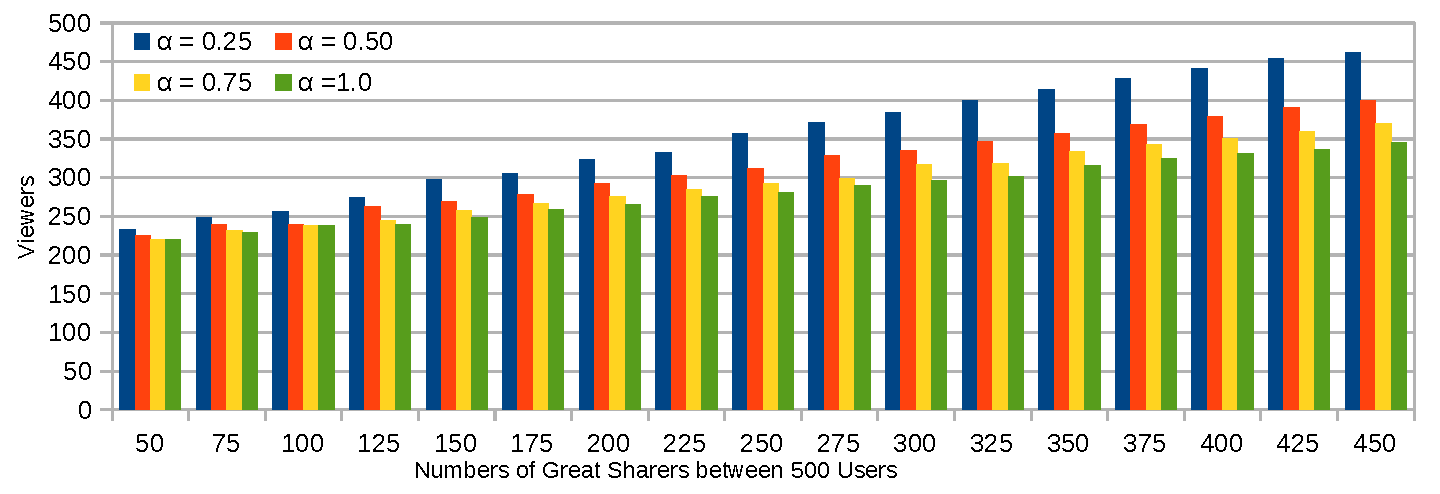
\includegraphics[width=1\textwidth]{charts/third-test-great-vs-little.pdf}
}
\caption{Grafico del risultato dell'ultimo test con forza della notizia pari a $0.50$, 
500 nodi totali e $\alpha$ del gruppo con bassa probabilità di condivisione = $0.75$}
\label{img:last_test_str_0_5}
\end{figure}

La figura \ref{img:last_test_str_0_5} mostra il risultato atteso, 
ovvero la crescita del numero di visualizzazioni sia al variare di $\alpha$ che all'aumentare 
dei nodi con alta probabilità di condivisione.
Si vuole inoltre porre l'attenzione su come con un valore di $\alpha$ 
molto basso ($0.2$) ed un numero di nodi con alta probabilità di condivisione pari a 150 corrisponda 
a $\approx$ 300 visualizzazioni totali, quasi le stesse ottenute da un valore di $\alpha$ = 1.0 e 325 nodi con 
alta probabilità di condivisione.















